%%%%Internal Cryogenics%%%%
\label{sec:fdsp-tc-internal-cryo}

The internal cryogenics comprises three sets of pipe distribution networks and two sets of sprayers. All pipes enter the cryostat from the top; some go all the way down to the floor, and others remain in the ceiling. On the floor are:
\begin{itemize}
\item \textbf{Argon gas distribution}: a set of pipes 
for \dword{gar}. These pipes are used only prior to filling to remove air 
in the cryostat. 
They will all have either a longitudinal slit or calibrated holes to distribute \dword{gar} uniformly along the length of the cryostat. 
We have run \dword{cfd} simulations showing that air will be removed from the system as long as \dword{gar} is flowing in at the right speed, calculated and experimentally verified as \SI{1.2}{m/hr} (vertical meters in the cryostat).  


\item \textbf{\dword{lar} distribution}: two sets of pipes are required for flowing 
\dword{lar} over a broad  range of flow rates. These pipes are used to fill the cryostat and, during steady state operations, to return the \dword{lar} from the purification system. The pipes have calibrated holes to return the \dword{lar} uniformly throughout the length of the cryostat which is very important to maintain uniform purity. 
Four pumps circulate the \dword{lar} inside the cryostat all of which operate initially to achieve purity. 
Once the target purity is achieved only one or two pumps remain in service. Individual pumps can be isolated for routine maintenance.
\end{itemize}

On the ceiling are:

\begin{itemize}
\item \textbf{Cool down sprayers}: Two sets of cool down sprayers are distributed along the long sides of each cryostat. One set distributes \dword{lar} using liquid sprayers that generate a conical profile of small droplets of liquid. The other set of sprayers distributes \dword{gar} to move the \dword{lar} droplets within the interior and thus cool down the detector and cryostat uniformly. These sprayers are being tested in \dword{pddp}. They are a variation of those implemented in \dword{pdsp}.
\end{itemize}

Figure~\ref{fig:internal-cryo-3D} shows the current layout of the internal cryogenics. 
%The current drawing of the internal cryogenics is presented in Figure~\ref{fig:internal-cryo-drawing}. 
The \dword{gar} pipes are in red, the \dword{lar} pipes in blue.

\begin{dunefigure}[Layout of the internal cryogenics piping]{fig:internal-cryo-3D}
  {Endview of the inside of the cryostat after the cryogenic piping has been installed. The \dword{gar} pipes used during the piston purge are in red and the pipes which return the purified \dword{lar} to the cryostat are in blue.}
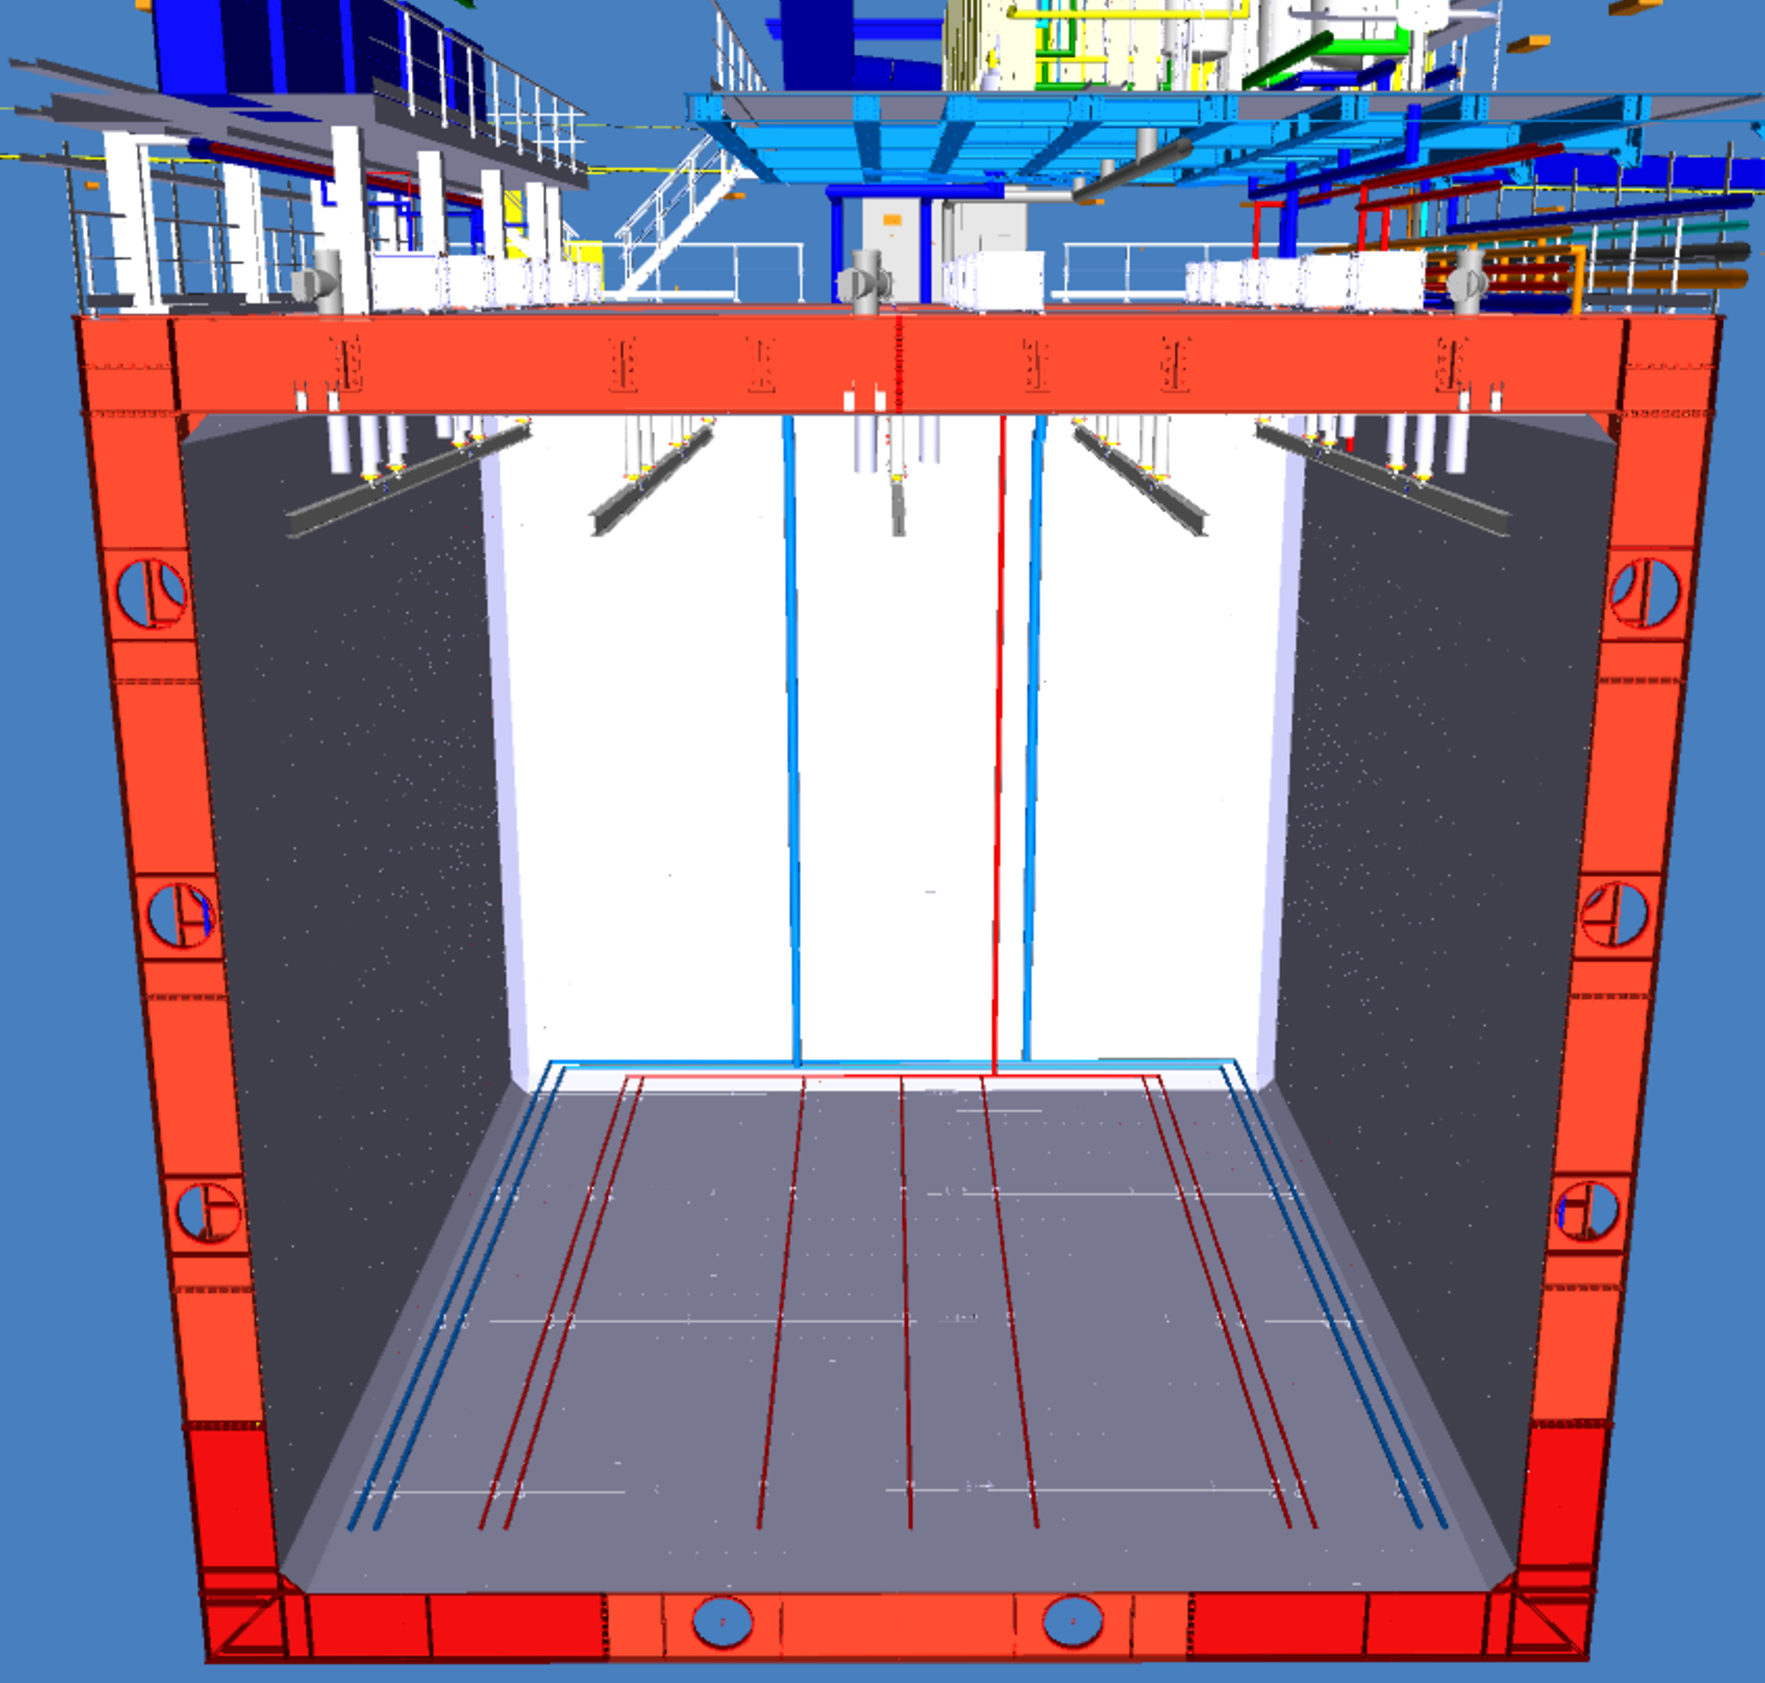
\includegraphics[width=.98\textwidth]{graphics/Internal-Piping-3D.pdf}
\end{dunefigure}


